\documentclass[conference]{IEEEtran}

\usepackage{cite}
\usepackage{url}

\ifCLASSINFOpdf
  \usepackage[pdftex]{graphicx}
  \DeclareGraphicsExtensions{.pdf,.jpeg,.png}
\else
  \usepackage[dvips]{graphicx}
  \DeclareGraphicsExtensions{.eps}
\fi
\graphicspath{{figures/}}
\usepackage[caption=false,font=footnotesize]{subfig}

%\usepackage[cmex10]{amsmath}
%\interdisplaylinepenalty=2500
%\usepackage{algorithmic}
%\usepackage{array}
%\usepackage{mdwmath}
%\usepackage{mdwtab}
%\usepackage{eqparbox}
%\usepackage{fixltx2e}
%\usepackage{stfloats}

% correct bad hyphenation here
% \hyphenation{op-tical net-works semi-conduc-tor}

\begin{document}
\title{Modeling speech production using the
  Neural Engineering Objects Framework NENGO2.0}

\author{\IEEEauthorblockN{Bernd J. Kr\"{o}ger}
\IEEEauthorblockA{Neurophoentics Group,\\
Department for Phoniatrics, Pedaudiology,\\
and Communication Disorders,\\
Medical School, RWTH Aachen University, Germany\\
Email: bkroeger@ukaachen.de}
\and
\IEEEauthorblockN{Trevor Bekolay and Chris Eliasmith}
\IEEEauthorblockA{Centre for Theoretical Neuroscience,\\
University of Waterloo, Canada\\
Email: \{tbekolay, celiasmith\}@uwaterloo.ca}}

\maketitle

\begin{abstract}
  A neurobiologically plausible model of speech production is
  introduced here using the NENGO neural simulator
  (\url{http://nengo.ca/}). It will be shown that this approach allows
  detailed modeling of temporal aspects of action selection and action
  execution in speech production. A preliminary architecture of our
  NENGO speech production model will be introduced and discussed in
  the second part of this paper. The first part focuses on an
  articulatory-acoustic model, generating acoustic speech signals on
  the basis of articulatory geome­tries. A mall set of functional
  articulatory control parameters is used in our approach. Motor
  planning is based here the concept of speech or vocal tract actions
  (Kr\"{o}ger et al. 2010, Cognitive Processing 11: 187-205). A
  2D-geometrical model is used and the acoustic speech signal is
  calculated using a reflection-type line analog model.
\end{abstract}

% no keywords

\IEEEpeerreviewmaketitle

\section{Introduction}

Different approaches exist for describing the speech production
hierarchy. Cortical processing starts with conceptualization of the
communicative act, followed by lexical retrieval of words, and its
syntactic processing. Subsequently a phonological sound sequence is
encoding for the planned utterance (e.g. \cite{levelt1999}). At lower
levels of speech production, the phonological representation activates
syllable-level motor plans mainly at premotor cortical areas, which is
followed by motor execution, involving primary motor areas,
cerebellum, basal ganglia, as well as the motor neuron system of
speech articulators \cite{riecker2005}. Subsequently, a temporal
succession of vocal tract shapes and the acoustic speech signal is
generated by the peripheral vocal tract system. Our model focuses on
lower levels of speech production and comprises a functional
articulatory-acoustic model, especially designed for speech learning.
Input units are speech or vocal tract actions
\cite{kroger1993,kroger2010}. These actions define a sequence of vocal
tract shapes. The most important information extracted from each vocal
tract shape, i.e. from each positioning of speech articulators, is the
shape of vocal tract cavities, which serves as basis for the
generation of the acoustic speech signal \cite{kroger1993}.

\section{The Action-Based Approach for Controlling Speech
  Articulation}

Based on previous work \cite{saltzman1989,goldstein2006}, we assume
\textit{vocal tract action units} (also called speech actions or
speech gestures) as the basic motor planning units in speech
production \cite{kroger2010}. From the viewpoint of speech learning it
is evident that babies in first year of lifetime babble a multitude of
\textit{gross vocal tract actions}, mainly leading to successions of
vocal tract opening and closing actions, sounding like e.g. [baba],
[dada] or [gaga] and so forth \cite{kroger2009,kroger2014}. Thus, we
can start by separating vocal tract \textit{opening actions} and vocal
tract \textit{closing actions}. Vocal tract opening actions also can
be called \textit{vocalic actions}, because they result in a
vowel-like sound. Vocal tract closing actions are also called
\textit{consonantal actions}, because they lead to a local vocal tract
constriction, e.g. produced by the lips, by the tongue dorsum, or by
the tongue tip. In addition babies already are capable of producing
\textit{velopharyngeal ab- and adduction actions} (lowering and
elevation of the velum), leading in a separation of nasal and
non-nasal sounds, and of producing \textit{glottal ab- and adduction
  actions} (ab- and adducting the vocal folds mainly by ab- and
adducting the arythenoids), leading to a separation of voiced and
voiceless sounds \cite{kuhl2004}. Vocal sounds produced so far are not
necessarily language specific but result from baby’s exploration of
the vocal tract (babbling period).

All types of vocal tract actions resulting from babbling are listed in
Table~\ref{tab:actions} and it is the main goal of speech learning i)
to fine tune these (gross) vocal tract actions with respect to
\textit{spatial} as well as to \textit{temporal intra-vocal tract
  action parameters}, in order to be capable later on to produce
different vowels and consonants of a specific target language and ii)
to fine tune the temporal coordination between different vocal tract
actions by varying \textit{inter-vocal tract action parameters} with
respect to the specific prosodic characteristics of that target
language. These parameters determine the temporal location of
consonantal, velopharyngeal and glottal actions with respect to
vocalic speech actions. An example for the temporal ordering of a
monosyllabic word produced by our control component is given in
Figure~\ref{fig:actions} (word ``palm''). In our current model, the
\textit{intra-action temporal control} as well as the
\textit{inter-action timing} is defined by values for the beginning
and ending of onset-, target- and offset-time interval for each vocal
tract action. These time instants are elucidated in
Figure~\ref{fig:actions} for all speech actions forming the word
``palm''. During \textit{onset time interval}, articulators move
towards the spatial action target, e.g. to lip closure in case of a
labial closing action or to an open vocal tract shape in case of the
vocalic action in ``palm''. This (partial) vocal tract target shape is
hold during \textit{target time interval} (e.g. hold of closure during
target interval of a consonantal closing action) and released at begin
of \textit{offset time interval}.

\begin{table}[!t]
\renewcommand{\arraystretch}{1.3}
\caption{Types of vocal tract actions, their spatial intra-vocal tract
  action parameters, and examples for potential speech sounds (symbols
  in parentheses []) or speech sound features which can be produced
  after learning a correct parameter specification.}
\label{tab:actions}
\centering
\begin{tabular}{l|p{2.5cm}|p{4cm}}
  type of action & spatial parameters & examples (after fine-tuning of
  actions)\\
  \hline
  vocalic & high-low & high: [i, u, y]; low: [a]\\
  ~ & back-front & back: [u]; front: [i, y]\\
  ~ & spread-rounded & spread [i]; rounded: [u, y]\\
  \hline
  consonantal & end-effector & lips: [b, p, f, m];
  tongue tip: [d, t, s, n, l]; tongue dorsum: [k, g]\\
  ~ & degree (type) of constriction &
  full closure: [b, p, m, d, t, n, k, g] (plosives and nasals) \newline
  near closure: [f, s, S] (fricatives) \newline
  lateral closure: [l]\\
  ~ & location of constriction & in case of tip: [s] in ``saw''
  vs. [S] in ``show''\\
  \hline
  velopharyngeal & abduction & nasal speech sounds: [m, n]\\
  ~ & adduction & non-nasal speech sounds (vowels, plosives, fricatives,
  ...)\\
  \hline
  glottal & abduction & voiceless speech sounds: [p, t, k, f, s, S]\\
  ~ & adduction & voiced speech sounds: [b, d, g, m, n, l] and all
  vowels\\
  pulmonic & pressure (resulting from movements of chest and diaphragm)
  & One action per utterance; constant pressure;
  degree of that pressure determines speech intensity of whole utterance
\end{tabular}
\end{table}

\begin{figure}[!t]
\centering
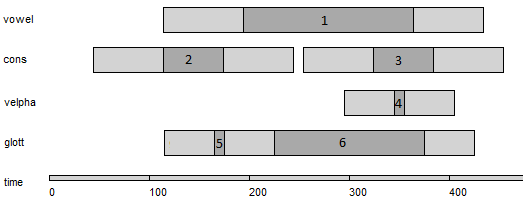
\includegraphics[width=\columnwidth]{actions}
\caption{Vocal tract action score of the word ``palm'' [pam]. Vocal
  tract actions are ordered with respect to four tiers (vocalic,
  consonantal, velopharyngeal, and glottal). Temporal location of
  onset (lightgray), target (darkgray), and offset time intervals
  (lightgray) for all six vocal tract actions of the word are shown.
  1: vocalic action with low spatial target position; 2: labial full
  closing action; 3: labial full closing action; 4: velopharyngeal
  abduction action; 5: glottal abduction action; 6: glottal adduction
  action. The offset time interval for action 5 is overlapped by the
  onset time interval of action 6. Time scale (bottom) is in msec.
  Thus, action 1 and 6 lead to [a], action 2 and 5 lead to [p], and
  action 3, 4, and 6 lead to [m]. The temporal overlap of vocal tract
  actions can also be called coarticulation.}
\label{fig:actions}
\end{figure}

\section{Control Parameters, Vocal Tract Shapes, and Area Functions}

Our set of articulatory control parameters is small but
\textit{functional} from the viewpoint of speech production: Three
vocalic parameters, i.e. \textit{front-back}, \textit{high-low}, and
\textit{spread-rounded} control the overall shape of the vocal tract
as is needed for the production of all vowels (examples are given in
Figure~\ref{fig:sagi}, top). The consonantal parameters \textit{lip
  adduction}, \textit{tongue tip elevation}, \textit{tongue body
  elevation} control \textit{degree (or type)} of consonantal
constrictions (e.g. full-closure in case of plosives or nasals, near
closure in case of fricatives, lateral closure in case of lateral).
Thus, while vocalic parameters control the whole shape of vocal tract,
only local parts of the vocal tract shape are controlled by the
consonantal parameters (e.g. lip region, tongue tip region, or tongue
dorsum region, see Figure~\ref{fig:sagi}, bottom). In addition the
parameters \textit{glottal abduction} and \textit{velopharyngeal
  abduction} control the positioning of vocal folds and of the velum
respectively.

While the \textit{shape of the vocal tract} in complex models is
generated on the basis of modeling muscular and tissue structures of
speech articulators (e.g. \cite{dang2004}), our approach is purely
geometrical. The contours of speech articulators are described by the
locations of a set of 14 contour points for upper lips, 17 points for
lower lips, 23 points for tongue, 15 points for hard palate, 34 points
for velum, and 23 points for pharynx wall, larynx, and epiglottis. The
locations of these contour points are obtained from static MRI scans
for three contours representing the (extremal) cardinal vowels [i, a,
u] (see \cite{kroger2005,kroger2004}). It is assumed that all vowel
shapes can be generated by interpolation from these extremal contours
using the three \textit{vocalic control parameters} introduced above.
In addition, extremal contours are generated for maximum labial
adduction and for maximum elevation of tongue tip as well as for
maximum elevation of tongue dorsum. Consonantal vocal tract shapes
within the local regions of the specific consonantal constriction are
interpolated between the current underlying vocalic tract shape and
the current consonantal extremal contours. Beside \textit{degree of
  constriction} (see above), one more parameter is needed in case of
tongue tip, controlling \textit{place of articulation}, in order to be
able to differentiate alveolar and postalveolar tongue tip
constrictions (e.g. [s] vs. [S], see Table~\ref{tab:actions}). The
exact location for tongue dorsum closure is controlled indirectly by
the current value of the vocalic front-back parameter.

\begin{figure*}[!t]
\subfloat[{[a]}]{
  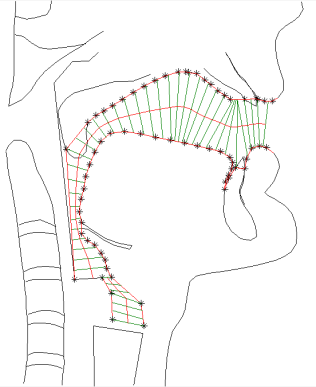
\includegraphics[width=0.2\textwidth]{sagi1}
  \label{fig:sagi1}
}
\hfil
\subfloat[{[i]}]{
  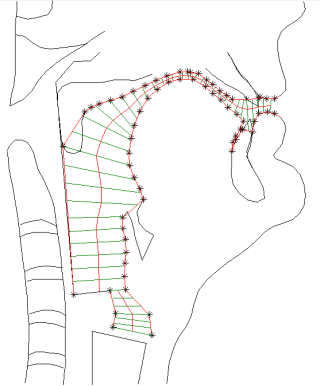
\includegraphics[width=0.2\textwidth]{sagi2}
  \label{fig:sagi2}
}
\hfil
\subfloat[{[u]}]{
  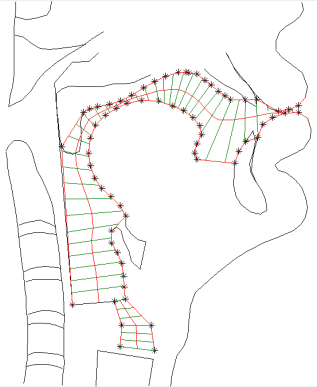
\includegraphics[width=0.2\textwidth]{sagi3}
  \label{fig:sagi3}
}
\hfil
\subfloat[?]{
  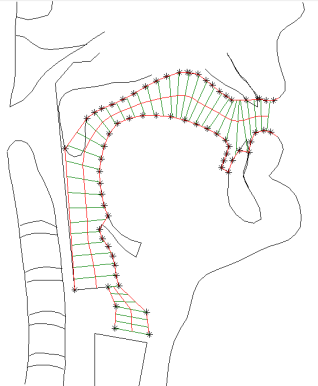
\includegraphics[width=0.2\textwidth]{sagi4}
  \label{fig:sagi4}
}

\subfloat[area function for {[a]}]{
  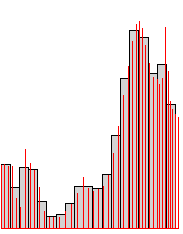
\includegraphics[width=0.2\textwidth]{sagi5}
  \label{fig:sagi5}
}
\hfil
\subfloat[lips closure]{
  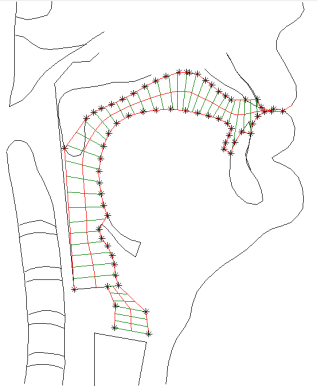
\includegraphics[width=0.2\textwidth]{sagi6}
  \label{fig:sagi6}
}
\hfil
\subfloat[tongue tip closure]{
  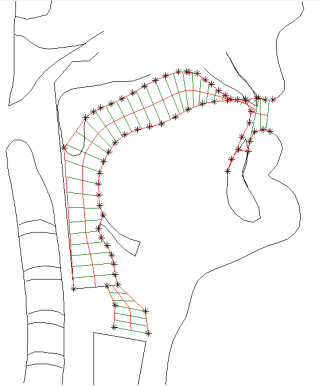
\includegraphics[width=0.2\textwidth]{sagi7}
  \label{fig:sagi7}
}
\hfil
\subfloat[tongue dorsum closure]{
  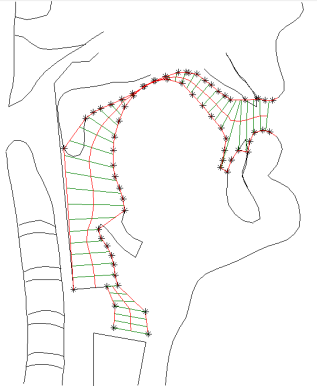
\includegraphics[width=0.2\textwidth]{sagi8}
  \label{fig:sagi8}
}
\caption{Top row: midsagittal views of low vowel [a],
  high-front-spread vowel [i], high back-rounded vowel [u]. Bottom row
  left: area function for vowel [a]. Bottom row right: midsagittal
  views of consonantal closures produced by lips, tongue tip, and
  tongue dorsum.}
\label{fig:sagi}
\end{figure*}

While no coarticulatory corrections are needed for the interpolation
of vocalic contours (i.e. lip rounding can be independently controlled
from tongue positioning without causing any problems in our
geometrical model), two coarticulatory corrections are needed in the
case of consonantal articulation. (i) In the case of producing a
labial constriction (increasing lip adduction), the front part of
tongue needs to be elevated, because lip adduction implies an
elevation of lower jaw. (ii) In the case of producing an apical
constriction (increasing tongue tip elevation), spatial coarticulation
needs to be high in case of high vowels. Here, the contour of
consonantal closure needs to be influenced strongly by the current
underlying vocalic vocal tract shape. This our model this problem is
solved by introducing different consonantal target shapes due to the
current vocalic coarticulation (see also \cite{kroger2004}).

For calculating the \textit{vocal tract area function} from a vocal
tract shape, a lower line, an upper line, and a midline is defined
(red lines in midsagittal views of Figure~\ref{fig:sagi}). Lower line
represents the front-low margin, upper line the back-high margin of
the vocal tract cavity (vocal tract tube) from larynx to lips. Midline
defines the midline for the airflow through the vocal tract tube from
glottis to lips. While the lower and upper line are defined by vocal
tract contour points (see black marks in Figure~\ref{fig:sagi}), the
calculation of the midline as well as of the green distance lines
(Figure~\ref{fig:sagi}) is done in a complex iteration procedure. A
set of \textit{42 distance lines} is defined, where these distance
lines are perpendicular to the midline and thus perpendicular to the
airstream within the vocal tract tube (green lines in sagittal views
of Figure~\ref{fig:sagi}). This set of distance lines is the basis for
calculating the area function (an example for an area function is
given in Figure~\ref{fig:sagi5}) for each vocal tract shape (cf.
\cite{perrier1992})

\section{Modeling Vocal Tract Acoustics}

Input for the calculation of the acoustic speech signal is area
function and glottal flow. The glottal flow is calculated using an
LF-model derivate \cite{veldhuis1998}. Flow and pressure values within
the vocal tract are calculated using a reflection-type line analog
\cite{liljencrants1985}. Here, the geometry of the vocal tract tube is
``digitized'' into a succession equidistant cylindrical tubes (see
gray columns, representing the area function in
Figure~\ref{fig:sagi5}). The length of each tube segment is 0.875 cm
in our case of 20 kHz sampling frequency for the acoustic signal. Flow
and pressure values are calculated for each tube segment at each time
instant. Acoustic and aerodynamic loss mechanisms including losses due
to sound radiation at mouth are included \cite{liljencrants1985}.
Because the length of the vocal tract and thus the number of tube
segments varies with respect to overall tube length (e.g. longer tract
length and thus more tube segments in case of [u] in comparison to [i]
or [a]), and because the reflection-type line analog cannot handle
varying tube length easily, the vocal tract shape over time is
calculated merely one time per glottal pulse (glottal period). The
resulting radiated sound signal (pulse response) is calculated over a
time interval of two glottal periods (Figure~\ref{fig:signal}) and is
overlayed pulse by pulse in time, in order to form the overall speech
sound signal.

\begin{figure}[!t]
  \begin{minipage}[b]{0.2\columnwidth}
    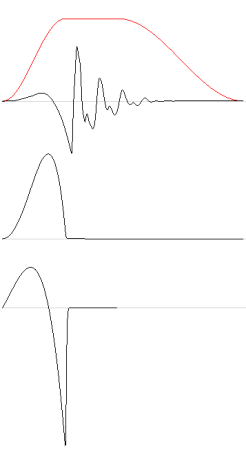
\includegraphics[width=\textwidth]{signal1}
  \end{minipage}
  \hfil
  \begin{minipage}[b]{0.8\columnwidth}
    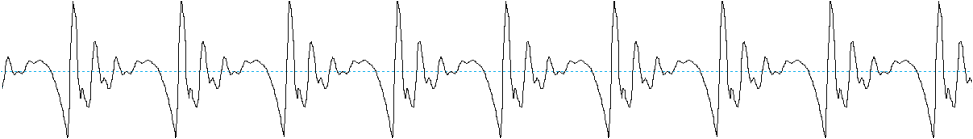
\includegraphics[width=\textwidth]{signal2}\\
    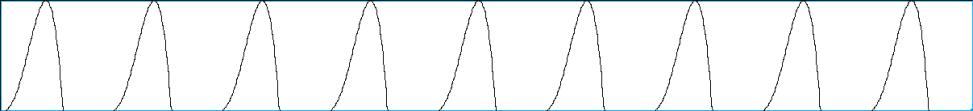
\includegraphics[width=\textwidth]{signal3}\\
    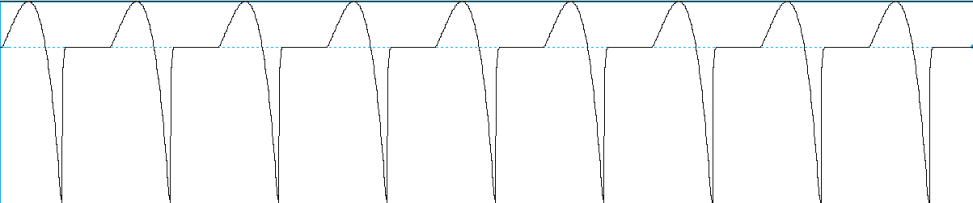
\includegraphics[width=\textwidth]{signal4}
  \end{minipage}
  \caption{Left side: single glottal pulse (middle: glottal flow;
    bottom: its time derivative for exactly one glottal period) and
    pulse answer for an [a], radiated from mouth (top); Right side
    top: acoustic speech signal, resulting from overlayed pulse
    answers; Middle: glottal flow waveshape for 9 glottal cycles;
    Bottom: first time derivative of glottal flow. The Hanning window
    for temporal overlay of pulse responses is asymmetric. Onset ends
    at time instant of maximum glottal excitation (i.e. negative peak
    of time derivative of glottal flow) and offset interval begins at
    end of glottal cycle. Right side signals are displayed using PRAAT
    software on basis of wav-signal output, generated by our
    synthesizer; left side signals are displayed from synthesizer
    software directly.}
\label{fig:signal}
\end{figure}

\section{The NENGO environment}

A NENGO (Neural ENGineering Objects; see \url{http://nengo.ca/}) is a
neural simulation environment capable of modeling for example visual
object recognition or copy drawing of manually drawn digits by
performing visual perception, cognitive tasks, as well as motor tasks
for controlling a two-joint arm \cite{eliasmith2012,eliasmith2013}.
These cognitive and sensorimotor tasks are performed on the basis of a
complex brain model which comprises many networks representing
cortical circuits, basal ganglia, thalamus, as well as peripheral
sensory processing and motor control. Each neural (sub-)network within
this approach is based on spiking model neurons, mainly LIF
(leaky-integrate-and-fire) neurons (\cite{eliasmith2013}, p. 35ff).
Moreover this simulation environment comprises a
cortex-basalganglia-thalamus-cortex loop capable of modeling action
selection and action execution as is needed in order to simulate for
example communi­cation behavior (e.g. question-answering scenarios).

We believe that this approach is helpful for modeling speech
acquisition and speech processing, because its action selection and
execution mechanisms can be extended or modified for modeling speech
acquisition (including face-to-face interaction between baby and
caretaker; see \cite{kroger2011}) as well as for adult speech
processing (i.e. production and perception). In the next section of
this paper, a preliminary architecture for speech processing is
introduced. The third section of this paper describes two simulation
experiments which highlight some key features of NENGO which are
important for speech processing: (1) simulation of syllable sequencing
and (2) simulation of action selection and execution in a listening
and articulatory reproduction task.

\section{The architecture of the speech production and perception
  model}

A speech processing model should comprise a cognitive component
(mental lexicon) as well as a sensorimotor component (speech action
repository SAR and a production-perception loop, see
\cite{kroger2009,kroger2014,kroger2012,kroger2011a,eckers2013,eckers2013a,kroger2010}).
It is a key feature of our ongoing work on modeling speech acqusition
and speech processing that phonological representations arise during
early phases of speech acquisition and are not predefined in the model
at the beginning of speech acquisition
\cite{kroger2009,kroger2014,kroger2011}. Lexical items (semantic as
well as phonological representations) as well as phonetic (i.e.
hypermodal sensorimotor) representations of syllables within the
speech action repository
\cite{kroger2012,kroger2011a,eckers2013,eckers2013a,kroger2010} can be
represented in NENGO using the semantic pointer architecture (SPA, see
\cite{eliasmith2013}, p. 77ff). The word ``semantic'' is not used in
NENGO in a narrow linguistics sense. Thus, semantic pointers are not
used exclusively to represent meanings of words, phrases or sentences
but can represent motor states as well, e.g. motor state (motor plan)
of a complete syllable or motor state (motor plan) of a
target-directed hand-arm gesture, or can represent sensory states,
e.g. auditory states of syllables, words or phrases, visual states,
etc. Thus, a semantic pointer in NENGO can be used to describe
discrete cognitive processing units as well as sensory and/or motor
states (e.g. phonetic states of syllables as are defined in SAR
\cite{kroger2012,kroger2011a,eckers2013,eckers2013a,kroger2010}).

An advantage of the NENGO framework is that it connects cognitive,
sensory, and motor sates. A comprehensive brain model including
cognitive, sensory and motor modules, called SPAUN
(\cite{eliasmith2012} and \cite{eliasmith2013}, p. 247ff) has been
developed based on NENGO. We believe that the motor system of SPAUN
can be augmented by a speech motor component, i.e. by a speech
articulator system, which can be implemented in parallel to the
already existing manual motor component. A discussion of similarities
and differences of controlling hand-arm motor system, articulator
motor system and facial motor system (in face-to-face communication
scenarios) is given in \cite{kroger2010}. Moreover the perceptual
system within SPAUN can be augmented by an auditory perceptual system
in order to allow speech acquisition and speech perception. This
auditory perceptual component can be implemented in parallel to the
already existing visual perceptual component (see
Figure~\ref{fig:model}).

\begin{figure}[!t]
\centering
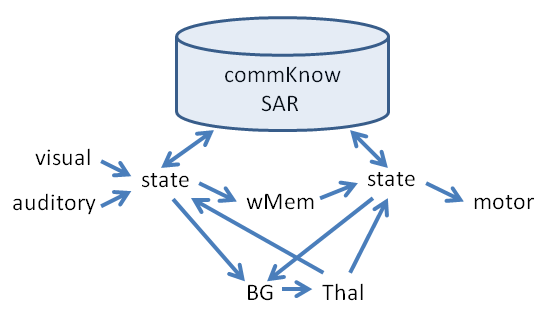
\includegraphics[width=\columnwidth]{model}
\caption{NENGO architecture for syllable and word processing.
  ``commKnow'' and ``SAR'' represent a neural long-term knowledge
  (communicative knowledge like mental lexicon and syllable action
  repository). ``wMem'' represents the working memory, ``BG'' the
  basal ganglia neural network, and ``Thal'' the thalamus neural
  network. Semantic pointers can be activated and processed in both
  state networks on the basis of audiovisual input (left state
  network: perceptual state network) or at the level of motor planning
  (right state network: action planning network; see also text).}
\label{fig:model}
\end{figure}

One further advantage of SPAUN is the neurobiological representation
of the cortex-basal ganglia-thalamus-cortex loop in order to model
action selection and control of perception-action tasks
(\cite{eliasmith2013}, p. 163ff). We believe that the concepts
introduced by \cite{eliasmith2013} for control of
visual-perception-manual-action tasks are applicable in a similar way
for auditory-perception-articulatory-speech-action tasks.

Sensorimotor as well as semantic knowledge concerning the production
and auditory state of syllables as well as of simple (mono-syllablic)
words, semantic as well as basic behavioral knowledge for face-to-face
communication in speech acquisition scenarios is stored in the SAR
(speech action repository) and commKnow (communicative knowledge)
module in form of predefined (i.e. learned) semantic pointers (Figure
4). Syllable state pointers (for example representing the syllables
``ba'', ``ga'', ``ga'', ...) as well as semantic pointers of
communication scenarios (for example representing actions like
``listen to a communication partner'', ``produce a syllable, word or
phrase'', ...) can be activated at the level of the state networks
(Figure 4), based on neural representations stored in long term memory
and based on actual audiovisual input (for example from a
communication partner / interlocutor). This information is processed
in working memory as well as in the
cortex-basal-ganglia-thalamus-cortex loop in order to generate and
activate motor plans (right state network) and in order to directly
control motor execution for articulation.

The size of the network components depends on the tasks which need to
be performed. In order to fulfill the tasks discussed in the next
section (syllable sequencing in speech production and control of
question-answering scenarios in speech communication), the size of
each cortical state network is 3000 model neurons each, the size of
the visual and auditory component as well as of the motor component is
300 model neurons each. The size of the recurrent network representing
the working memory is 1000 model neurons. The basal ganglia comprises
5 subnetworks with 600 model neurons each (3000 model neurons in
total, see \cite{eliasmith2013}, p. 164ff). The thalamus is
represented by a network of 750 model neurons (see
\cite{eliasmith2013}, p. 169ff).

\section{Discussion and Further Work}

First steps in the direction of using NENGO (\url{http://nengo.ca/})
in order to model speech acquisition and speech processing are
described in this paper. The NENGO framework seems to be advantageous
for modelling speech acquisition and speech processing because this
approach includes modelling of time as well as internal neural noise
generation due to use of LIF neurons in a natural and straight forward
way. This allows us to model aspects of speech acquisition and speech
processing which are beyond the scope of other approaches. Especially
aspects of face-to-face communication in speech acquisition due to
perception-action routing in the brain and specific aspects of speech
disorders due to different degrees of internal neural noise excitation
can now be investigated now in more detail.

In addition a functional articulatory-acoustic model has been
introduced. This model is designed for modeling the learning processes
for intra- and inter-speech action parameters, i.e. for fine-tuning of
action targets, for action onset-, target-, and offset-interval
lengths as well as for establishing the temporal relation between
different speech actions, forming a syllable or word (cf. babbling and
imitation training \cite{kroger2009,kroger2014}). Because these
simulations demands the generation of an abundance of speech items,
our model is designed for generating speech items nearly in real time.
Integrating nasal tract and noise sources for the generation of nasals
and fricatives respectively will be done in near future. A perceptual
evaluation of speech items produced by our model will follow.

\IEEEtriggeratref{5}

\bibliographystyle{IEEEtran}
\bibliography{kroger}

\end{document}
